\chapter{Cwiczenie 4 - czwórnik CLR}

\section{Polecenie}

Zbudować czwórnik CLR. Zmierzyć jego charakterystyke amplitudową i fazową dla sygnałów sinusoidalnych. Wyznaczyć wartość częstotliwości rezonansowej i porównać z wartością teoretyczną.

\section{Montaż układu}

Zmontowano układ używając (wartość indukcji cewki odczytana została z płytki RLC): 
\begin{gather}
    \textbf{R = 3.9k}\boldsymbol{\Omega} \\
    \textbf{C = 209.6nF} \\
    \textbf{L = 25.8mH}
\end{gather}
Posługując się trójnikiem rozdzielono wejście tak, aby na oscyloskopie można było obserwować sygnał wejściowy oraz wyjściowy:
    \begin{figure}[h]
        \centering
        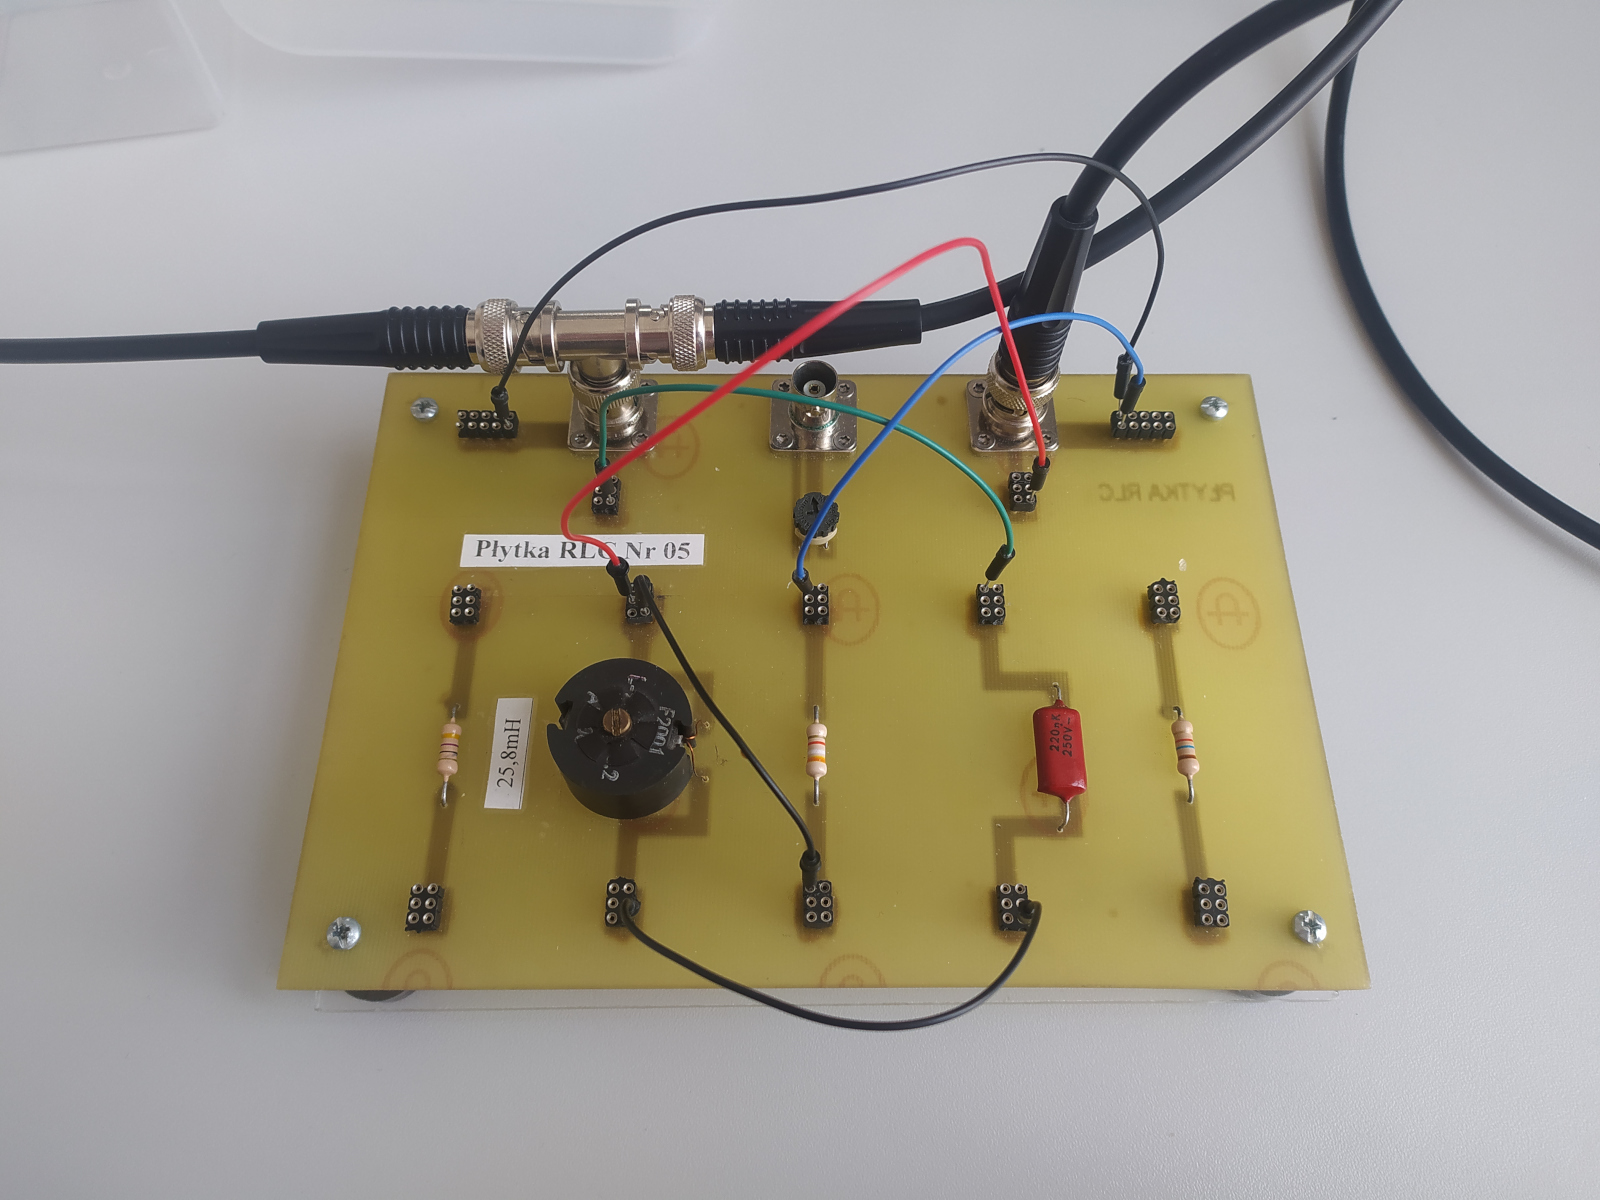
\includegraphics[scale=0.15]{img_phone/IMG_20220330_114556_smaller.jpg}
        \caption{Zmontowany czwórnik CLR}
        \label{fig:builtCR}
    \end{figure}

\section{Teoretyczne wyliczenia}

\begin{itemize}
    \item Wyliczona teoretyczna częstość rezonansowa oraz częstotliwość wyniosła:
        \begin{gather}
            \omega = \frac{1}{\sqrt{LC}} \approx 13598,6Hz = \textbf{13.5986kHz} \\
            f_0 = \frac{\omega}{2\pi} = \frac{13.5986kHz}{2\pi} \approx \textbf{2164Hz}
        \end{gather}
\end{itemize}

\newpage

\section{Pomiary}

\begin{itemize}
    \item Na układ podawano sygnał sinusoidalny o amplitudzie \textbf{2V} i różnej częstotliwości, docelowo częstotliwość $\in$ \textbf{$\langle$10;4000$\rangle$Hz}
    \item Ze względu na brak czasu, pomiary nie są kompletne. \\
    Nie udało się eksperymentalnie zauważyć punktu w którym występuje rezonans. \\
    Należałoby przeprowadzić dodatkowe pomiary dla częstotliwości bliskich teoretycznej (w tym przypadku około \textbf{$\langle$2000;2400$\rangle$Hz}) oraz większych niż teoretyczna.
    \item Zaobserwowano i zmierzono zależności dla częstotliwości mniejszych od wyliczonej teoretycznie.
    \item \textcolor{purple}{Przeprowadzone pomiary w postaci tabeli}:
        \begin{center}
            \Large %tabelka Uwe Uwy phi
            \label{poprawa:pomiary_CLR}
            \begin{tabular}{|>{\columncolor[gray]{0.8}}c|>{\columncolor[gray]{0.8}}c|c|>{\columncolor[gray]{0.8}}c|c|}
                 \hline
                 $f$ [Hz] & $U_{we}$ [V] & $U_{wy}$ [V] & $\frac{U_{wy}}{U_{we}}$ &  $\phi$ [$\degree$] \\
                 \hline
                 10 & 2 & 0.105 & 0.05 & -89.99 \\
                 \hline
                 25 & 2 & 0.256 & 0.128 & -83.25 \\
                 \hline
                 50 & 1.99 & 0.488 & 0.244 & -75.7 \\
                 \hline
                 100 & 1.99 & 0.88 & 0.44 & -63.77 \\
                 \hline
                 268.3 & 1.97 & 1.58 & 0.8 & -35.32 \\
                 \hline
                 300 & 1.97 & 1.65 & 0.837 & -31.18 \\
                 \hline
                 380.8 & 1.96 & 1.75 & 0.892 & -25.69 \\
                 \hline
                 500 & 1.96 & 1.84 & 0.938 & -20.04 \\
                 \hline
                 709 & 1.96 & 1.87 & 0.954 & -15.08 \\
                 \hline
                 985 & 1.95 & 1.87 & 0.959 & -10.97 \\
                 \hline
            \end{tabular}
        \end{center}
    
    \item Zrzuty z oscyloskopu przeprowadzonych pomiarów:
        \begin{figure}[H]
            \centering
            \begin{subfigure}[h]{0.4\textwidth}
                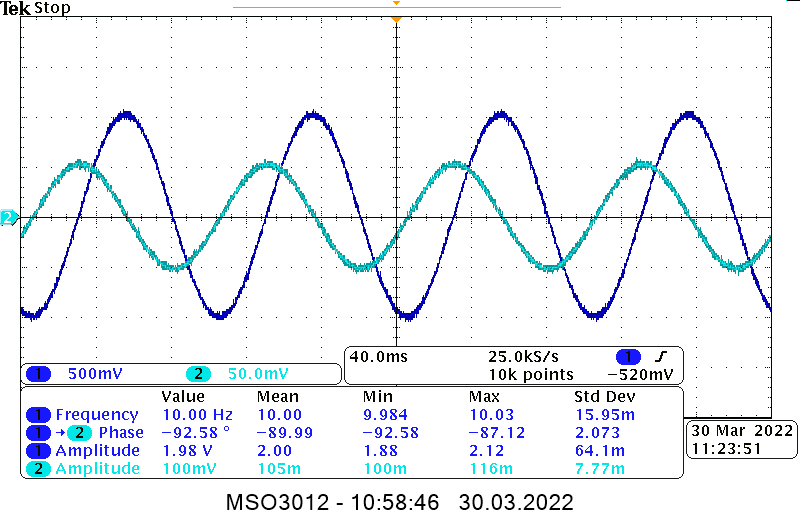
\includegraphics[width=\textwidth]{img_osciloscope/CLR/CLR_10Hz_cropped.png}
                \caption*{10Hz}
            \end{subfigure}
            \begin{subfigure}[h]{0.4\textwidth}
                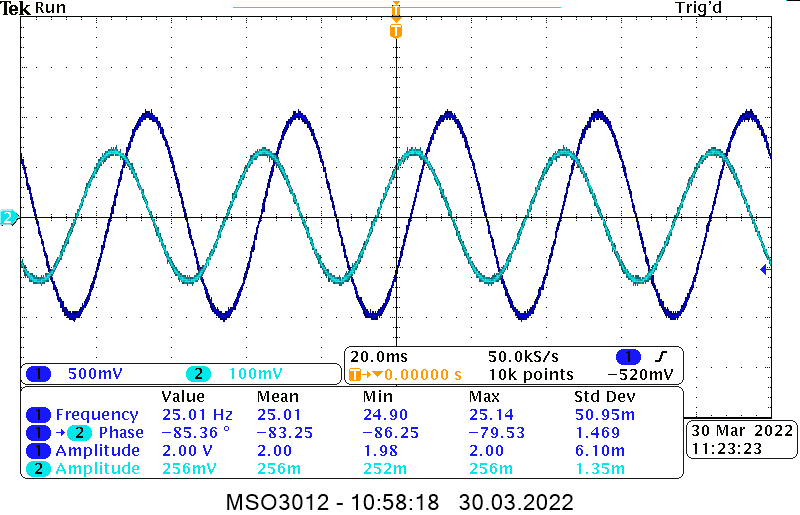
\includegraphics[width=\textwidth]{img_osciloscope/CLR/CLR_25Hz_cropped.png}
                \caption*{25Hz}
            \end{subfigure}
        \end{figure}
        \begin{figure}[H]
            \centering
            \begin{subfigure}[h]{0.4\textwidth}
                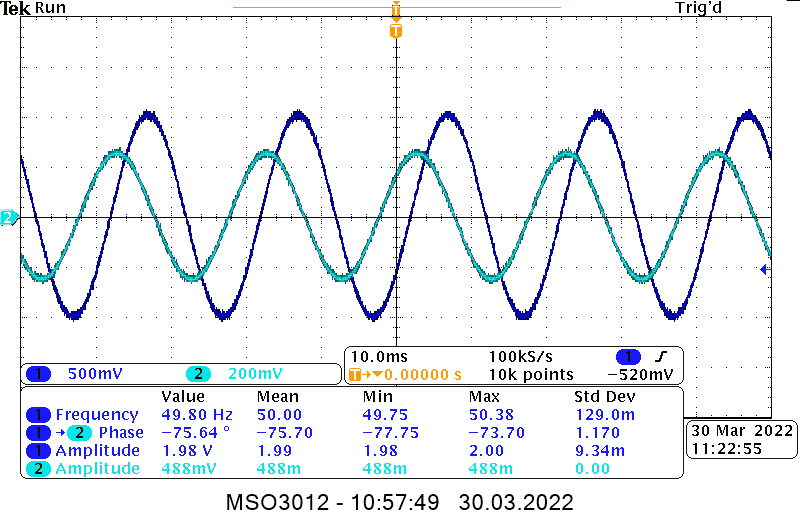
\includegraphics[width=\textwidth]{img_osciloscope/CLR/CLR_50Hz_cropped.png}
                \caption*{50Hz}
            \end{subfigure}
            \begin{subfigure}[h]{0.4\textwidth}
                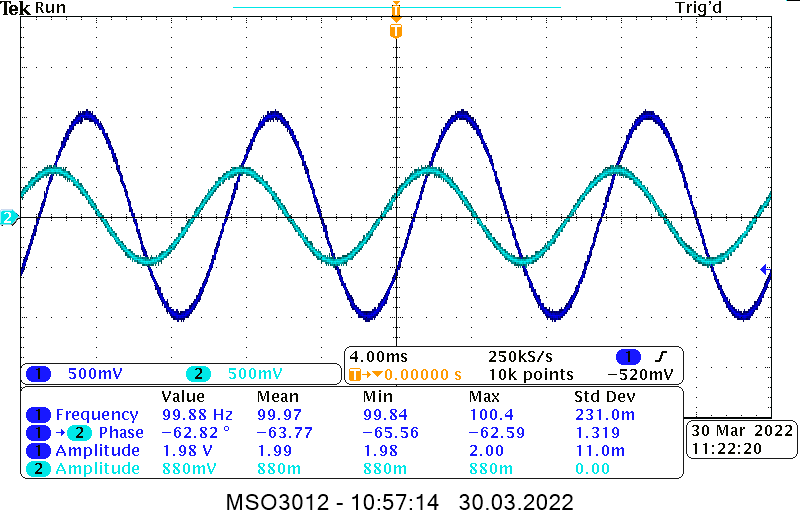
\includegraphics[width=\textwidth]{img_osciloscope/CLR/CLR_100Hz_cropped.png}
                \caption*{100Hz}
            \end{subfigure}
        \end{figure}
        \begin{figure}[H]
            \centering
            \begin{subfigure}[h]{0.4\textwidth}
                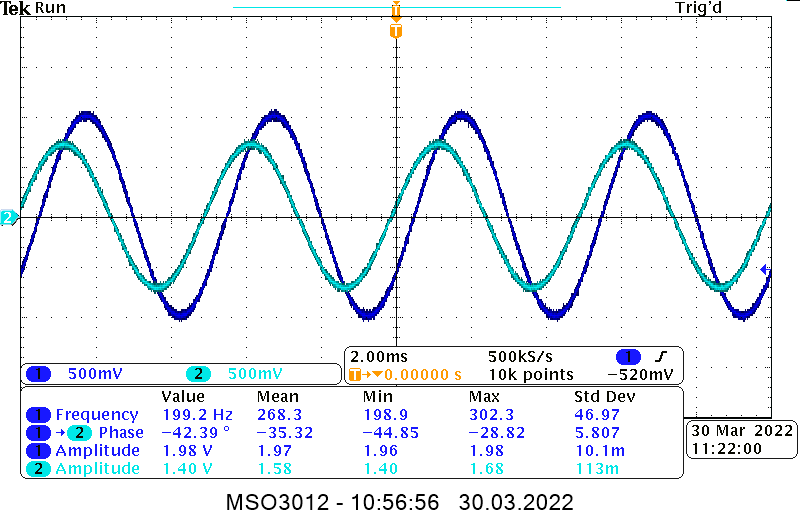
\includegraphics[width=\textwidth]{img_osciloscope/CLR/CLR_200Hz_cropped.png}
                \caption*{200Hz}
            \end{subfigure}
            \begin{subfigure}[h]{0.4\textwidth}
                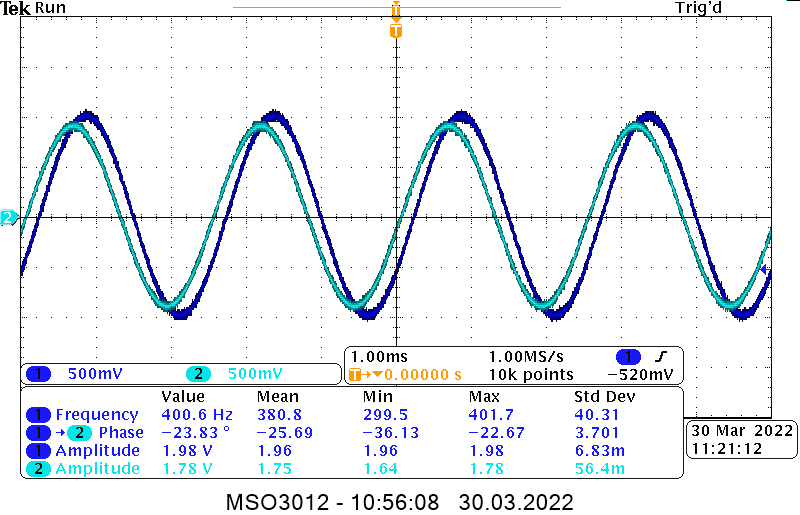
\includegraphics[width=\textwidth]{img_osciloscope/CLR/CLR_400Hz_cropped.png}
                \caption*{400Hz}
            \end{subfigure}
        \end{figure}
        \begin{figure}[H]
            \centering
            \begin{subfigure}[h]{0.4\textwidth}
                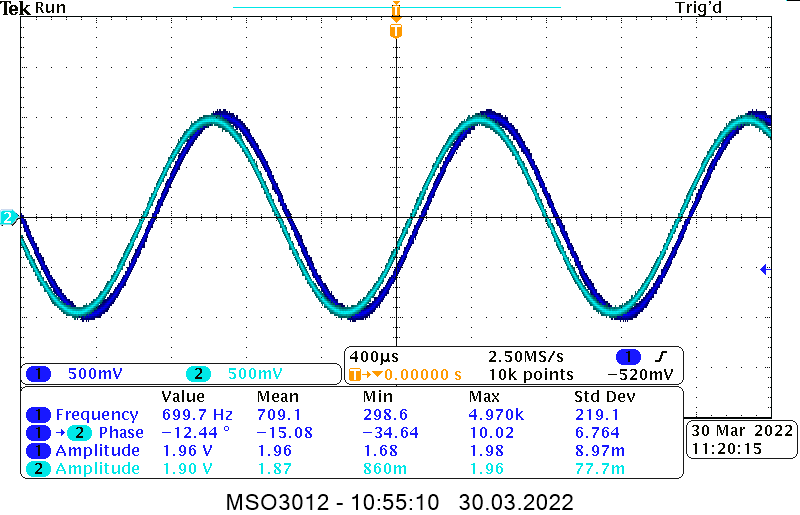
\includegraphics[width=\textwidth]{img_osciloscope/CLR/CLR_700Hz_cropped.png}
                \caption*{700Hz}
            \end{subfigure}
            \begin{subfigure}[h]{0.4\textwidth}
                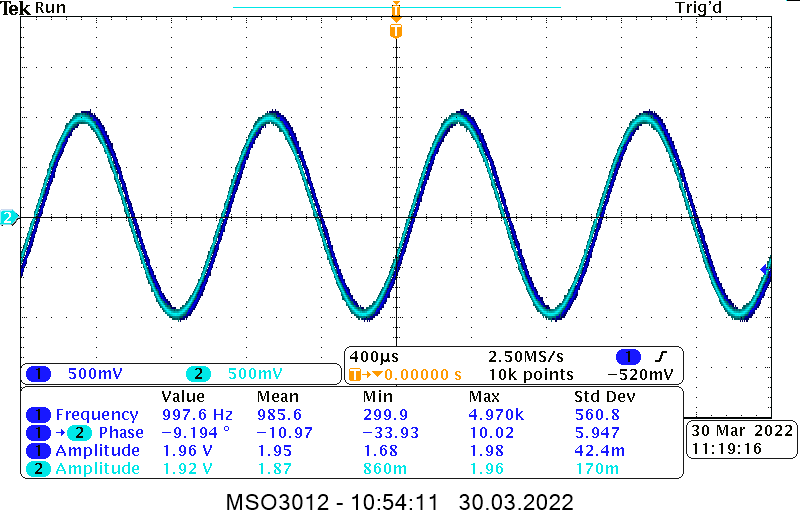
\includegraphics[width=\textwidth]{img_osciloscope/CLR/CLR_1000Hz_cropped.png}
                \caption*{1000Hz}
            \end{subfigure}
        \end{figure}
\end{itemize}

\section{Charakterystyki częstotliwościowe}

\begin{itemize}
    \item Ze względu na niekompletność pomiaru całkowite zbadanie charakterystyk amplitudowej oraz fazowej nie było możliwe.
    
\end{itemize}